\documentclass[tikz,border=10pt]{standalone}
\usetikzlibrary{calc}
\begin{document}
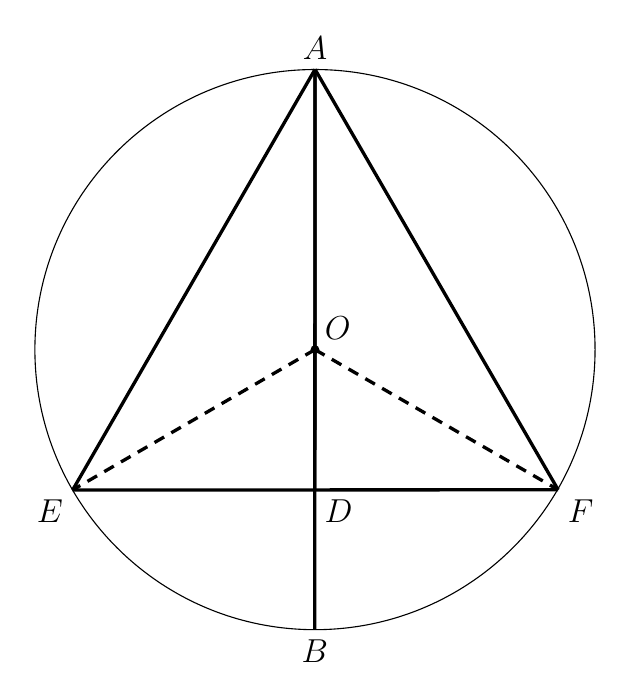
\begin{tikzpicture}[line join=round, font=\fontsize{12}{14.4}\selectfont]
\coordinate (A) at (-0.011,3.567);
\coordinate (B) at (-0.015,-3.551);
\coordinate (D) at (-0.015,-1.774);
\coordinate (F) at (3.076,-1.772);
\coordinate (O) at (-0.012,0.008);



\coordinate (E) at (-3.089,-1.774);


\draw[thin, black] (O) circle (3.557);


\draw[line width=1.2pt] (A) -- (B);
\draw[line width=1.2pt] (E) -- (D) -- (F);
\draw[line width=1.2pt] (A) -- (E);
\draw[line width=1.2pt] (A) -- (F);
\draw[line width=1.2pt] (A) -- (O);
\draw[line width=1.2pt] (D) -- (O);
\draw[line width=1.2pt] (B) -- (D);


\draw[line width=1.2pt, dash pattern=on 4pt off 3pt] (O) -- (E);
\draw[line width=1.2pt, dash pattern=on 4pt off 3pt] (O) -- (F);


\fill (O) circle (1.600pt);


\node[above] at (A) {$A$};
\node[below] at (B) {$B$};
\node[above right] at (O) {$O$};
\node[below right] at (D) {$D$};
\node[below left] at (E) {$E$};
\node[below right] at (F) {$F$};
\end{tikzpicture}
\end{document}